\par These notes are entirely based on the material of the course Computational Mathematics for Learning and Data Analysis held by Professor Antonio Frangioni and Professor Federico Poloni at University of Pisa. The course is part of the M.Sc. degree in Computer Science.

\section{Mathematical Background}
\subsection{Notations and Nomenclatures}
\par Let's start with introducing some notations and nomenclatures that we are going to use throughout this book. Given a set $\mathcal{X}$, that we call \textbf{feasible region}, and a function $f : \mathcal{X} \rightarrow \mathbb{R}$, that we call \textbf{objective function}, we want to find the solution to the following problem:
\begin{equation}
    f_{*} = \min_{x \in \mathcal{X}}\ \{f(x)\}
    \label{eq:opt_problem_def}
\end{equation}
where $f_{*}$ is called \textbf{optimal value}. The argument $x$ that \textit{minimises} the objective function $f$ is called \textbf{optimal solution}. It is generally denoted with $x_{*}$.\\[5px]
%
\underline{Note that}: $f_{*}$ lives in the output space while $x$ lives in the input space. This is going to be very important where we speak about convergence of the various algorithms that we will see during this brief journey.\\[5px]
%
Obviously, from the moment that we are minimising the function $f$, we have the following property:
\[
    \forall\ x \in \mathcal{X}\ f(x) \geq f(x_{*})
\]
Here again, note that we do not state any ordering relation in the input space; $x$ may be larger, equal or even smaller than $x_{*}$.
\par As we will see in the next chapters, we often employ \textit{iterative methods} for finding the optimal value/optimal solution. Applying an iterative method implies producing a certain sequence of the form $x_1, x_2, ...$ that will bring us to the optimum solution; and thus to the optimal value. Typically we cannot hope to get exactly to $f_{*}$, what we hope instead is to get \textit{as close as possible} to it. Accordingly, limits are very important to us.
We say that:
\begin{equation}
    \lim_{i \rightarrow \infty} x_i = x \iff \forall \epsilon > 0\ \exists h : |x_i - x| \leq \epsilon\ \forall i \geq h
    \label{eq:limit_def}
\end{equation}
In other words, the sequence $\{x_i\}$ converges to $x$, written as $\{x_i\} \rightarrow x$, if and only if... the rest of the formula :). Just kidding. So we were saying, the sequence $\{x_i\}$ converges to $x$ if and only if for \textit{any} tiny number $\epsilon$ that we can choose (as long as it is greater than 0), at some point in our sequence, starting from the number $x_h$, all the numbers in it will be at distance at most $\epsilon$ from $x$.
\par Not all sequences have the limit. For instance think of $(-1)^i$. This sequence does not converge to neither of -1, 0 or 1. This is the reason why we introduce the concept of \textbf{infima} and \textbf{suprema}, or respectively $\liminf$ and $\limsup$. We define the following two quantities:
\[
    \{x_i\} \rightarrow \underbar{$x$}_i = \inf\{x_h : h \geq i\}
\]
and
\[
    \{x_i\} \rightarrow \bar{x}_i = \sup\{x_h : h \geq i\}
\]
Now if we take the sequence of $\{\underbar{x}_i\}$ we are sure that $\underbar{x}_1 \leq \underbar{x}_2 \leq \underbar{x}_3 \leq ...$ and the sequence of $\{\bar{x}_i\}$ we are sure that $\bar{x}_1 \geq \bar{x}_2 \geq \bar{x}_3 \geq ...$. Accordingly, they have a limit! So we can speak about inferior and superior limit of a certain sequence $\{x_i\}$. We have the following equality:
\begin{align}
    &\liminf_{i \rightarrow \infty} x_i = \lim_{i \rightarrow \infty}\inf\{x_h : h \geq i\} = \lim_{i \rightarrow \infty} \underbar{x}_i\\
    &\limsup_{i \rightarrow \infty} x_i = \lim_{i \rightarrow \infty}\sup\{x_h : h \geq i\} = \lim_{i \rightarrow \infty} \bar{x}_i
    \label{eq:liminf_limsup_def}
\end{align}
Now obviously $\bar{x}_i \geq \underbar{x}_i$. But if these two quantities are equal, then we are sure that the limit of the sequence exists:
\[
    \lim_{i \rightarrow \infty} x_i = v \iff \liminf_{i \rightarrow \infty} x_i = v = \limsup_{i \rightarrow \infty} x_i
\]
%
\par Now the life would be pretty straightforward and we would not need to study optimisation if we worked just with single numbers, i.e. in $\mathbb{R}$. We need to scale.
%
\subsection{Euclidean Space \texorpdfstring{$\mathbb{R}^n$}{Rn}}
\par We will mostly use function that operate on vectors not numbers. We need to define the space in which these vectors have some meaning. We thus define the \textbf{Euclidean Space} as the Cartesian product of $n$ one dimensional spaces $\mathbb{R}$:
\begin{equation}
    \mathbb{R}^n = \underbrace{\mathbb{R} \times ... \times \mathbb{R}}_{n\ \text{times}}
    \label{eq:euclidean_space}
\end{equation}
The elements of this space are vectors of $n$ components, i.e. $x \in \mathbb{R}^n = [x_1, ..., x_n]$.\\[5px]
\underline{\textbf{Note}}: during this book we will always assume to work with \textbf{column vectors}. When we use \textbf{row vectors} we will use the transposition sign.\\[5px]
\par The Euclidean space is \textbf{closed} under summation and scalar multiplication. This means that whenever we take two vectors and we sum them, or we take a constant $\alpha$ and we multiply all the components of a vector with $\alpha$, we will always get a new vector that is for sure still in our Euclidean space.
\par The Euclidean space is a \textbf{finite} vector space: this means that each $x \in \mathbb{R}^n$ can be obtained from a \textbf{finite basis}. A basis is a set of vectors such that for whatever vector $x$ in the space, we can somehow linearly combine the vectors from the basis to obtain $x$. Linearly combine means summations and scalar multiplications.
\par The Euclidean space is \textit{not a totally ordered set}. We do not have a natural concept of which one comes first.
\par Since we will work a lot with distances we also need to define the concept of distance in this space. Before talking about the distance we need to introduce a very important concept that we will use constantly. \textbf{The norm}. We define Euclidean norm as:
\begin{equation}
    \lVert x \rVert = \sqrt{\sum_{i=1}^n x_i^2}
    \label{eq:2norm_def}
\end{equation}
Some of the properties of the Euclidean norm are:
\begin{itemize}
    \item $\lVert x \rVert \geq 0$ $\forall x \in \mathbb{R}^n$ with 0 only in case that $x$ is the zero vector
    \item $\lVert \alpha x \rVert = |\alpha| \lVert x \rVert$ $\forall x \in \mathbb{R}^n$ $\forall \alpha \in \mathbb{R}$
    \item $\lVert x+y \rVert \leq \lVert x \rVert + \lVert y \rVert$ $\forall x,y \in \mathbb{R}^n$. This property is called \textbf{triangular inequality}.
\end{itemize}
The norm function is nothing more than a simple function that maps vectors to numbers (also matrices to numbers). Apart from the norm we have defined in the equation \ref{eq:2norm_def}, we have also:
\begin{itemize}
    \item 0-norm $\lVert . \rVert_0 = |i : |x_i| > 0|$, i.e. the cardinality of the set of all non zero components in the vector $x$
    \item 1-norm $\lVert . \rVert_1 = \sum_{i=1}^n |x_i|$
    \item $\infty$-norm $\lVert . \rVert_\infty = \max_{i \in I}\{|x_i|\}$
\end{itemize}
All these norms (including 2-norm) are the special cases of the unique definition of the p-norm:
\begin{equation}
    \lVert x \rVert_p = \Big(\sum_{i=1}^n |x_i|^p\Big)^{\frac{1}{p}}
    \label{eq:p_norm}
\end{equation}
In figure \ref{fig:norms} we show how the function of the norm changes as we augment $p$. Note that for $p \geq 1$ we have a convex function while for $p < 1$ we have a concave function.
\begin{figure}
    \centering
    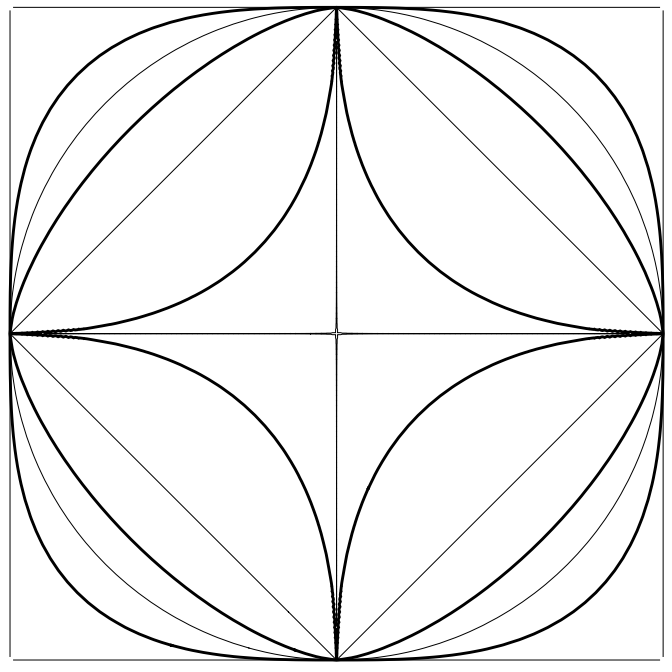
\includegraphics[scale=0.4]{figures/1/1-norms.png}
    \caption{The various types of norms}
    \label{fig:norms}
\end{figure}
\par It is not very important which norm we are using since all of them are topologically equivalent. This means that whatever two norms we choose, there is a simple linear relation between them:
\begin{equation}
    \forall\ \lVert . \rVert_x, \lVert . \rVert_y\ \exists\ 0 < \alpha < \beta : \alpha \lVert . \rVert_y \leq \lVert . \rVert_x \leq \beta \lVert . \rVert_y
    \label{eq:norm_equivalence}
\end{equation}
Accordingly, we are free to work with whatever norm. We will generally use the two norm, unless stated otherwise.
\par Another concept we have to introduce before defining the distance in the Euclidean space is the \textbf{scalar product} between two vectors. We define the scalar product as:
\begin{equation}
    \langle x,y \rangle = y^{T}x = \sum_{i=1}^n = x_i y_i
    \label{eq:scalar_product}
\end{equation}
Like the norm function, the scalar product is a simple function that takes two vectors and returns the value, i.e. $\langle.\rangle : \mathbb{R}^n \times \mathbb{R}^n \rightarrow \mathbb{R}$. It satisfies the following properties ($\forall\ x,y,z \in \mathbb{R}^n, \forall\ \alpha \in \mathbb{R}$):
\begin{itemize}
    \item $\langle x, y \rangle = \langle y, x \rangle$ (symmetry)
    \item $\langle x, y \rangle \geq 0$
    \item $\langle x, x \rangle = 0 \iff x = 0$
    \item $\langle \alpha x, y \rangle = \alpha \langle x, y \rangle$
    \item $\langle x + y, z \rangle = \langle x, z \rangle + \langle y, z \rangle$
    \item $\langle x, x \rangle = \lVert x \rVert^2$ (only for $\lVert . \rVert_2$)
    \item $\langle x, y \rangle^2 \leq \langle x, x \rangle \langle y, y \rangle = \lVert x \rVert^2 \lVert y \rVert^2$. This is a very important property and it is called \textbf{Cauchy-Schwarz inequality}
\end{itemize}
The scalar product have another definition, the one that uses the cosine function:
\begin{equation}
    \langle x,y \rangle = \lVert x \rVert \lVert y \rVert \cos \theta
    \label{eq:scalar_product_cos}
\end{equation}
From this definition it is clear that when two vectors are perpendicular to each other then the scalar product is 0 (figure \ref{fig:scalar}).
\begin{figure}
    \centering
    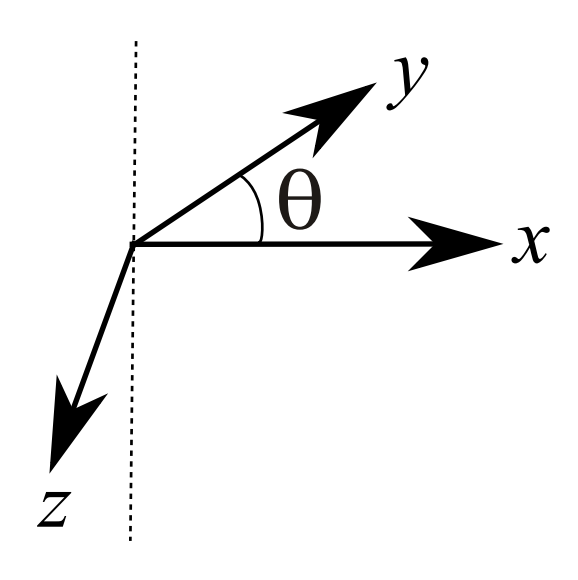
\includegraphics[scale=0.4]{figures/1/2-scalar.png}
    \caption{Angle $\theta$ between $x$ and $y$}
    \label{fig:scalar}
\end{figure}
When the two vectors point to the same direction then the scalar product is $> 0$. Cosine of an angle that is between 0 and $\frac{\pi}{2}$ is positive, thus the scalar product is positive (the norms are always $\geq 0$). This will be very useful when we will speak about various descent methods for unconstrained optimisation.
\par We are now ready to introduce the \textbf{Euclidean distance}. The Euclidean distance between $x \in \mathbb{R}^n$ and $y \in \mathbb{R}^n$ is defined as:
\begin{equation}
    d(x,y) = \lVert x - y \rVert = \sqrt{\sum_{i=1}^n(x_i - y_i)^2}
    \label{eq:euclidean_distance}
\end{equation}
The euclidean distance satisfies the following properties ($\forall\ x,y,z \in \mathbb{R}^n$ and $\forall\ \alpha \in \mathbb{R}$):
\begin{itemize}
    \item The distance between two vectors is always $\geq 0$: $d(x,y) \geq 0$
    \item $d(\alpha x, y) = |\alpha|d(x,y)$
    \item $d(x,y) \leq d(x,z) + d(z,y)$ (triangular inequality)
\end{itemize}
So the distance between two vectors is given by the norm of the vector difference between them.
\par We concept of Euclidean distance is useful for defining a very important mathematical object in optimisation.
%
\subsection{Ball, Interior, Boundary and Bounded sets}
\begin{definition}
    Given a centre $x \in \mathbb{R}^n$ and a radius $r > 0 \in \mathbb{R}$, we call \textbf{Ball}:
    \[
        \mathcal{B}(x,r) = \{y \in \mathbb{R}^n : d(x,y) \leq r\}
    \]
    \label{def:ball}
\end{definition}
Having these new mathematical objects, we can restate the concepts of converging sequences as:
\[
    \{x_i\}_{i \rightarrow \infty} \rightarrow x \iff \forall\epsilon > 0\ \exists h : d(x_i,x) \leq \epsilon\ \forall i \geq h
\]
or
\[
    \{x_i\}_{i \rightarrow \infty} \rightarrow x \iff \forall\epsilon > 0\ \exists h : x_i \in \mathcal{B}(x,\epsilon)\ \forall i \geq h
\]
or even
\[
    \lim_{i \rightarrow \infty} d(x_i,x) = 0
\]
Why we are so interested in these sequences of points? Because if we consider the optimisation problem again:
\[
    f_{*} = \min_{x \in \mathcal{X}}\ \{f(x)\}
\]
we want to construct the so called \textit{minimising sequence} $\{x_i\}_{i \rightarrow \infty}$ such that $\{f(x_i)_{i \rightarrow \infty}\} \rightarrow f_{*}$.\\
Note again (again, yes) that $\{f(x_i)_{i \rightarrow \infty}\} \rightarrow f_{*} \centernot\Rightarrow \{x_i\}_{i \rightarrow \infty} \rightarrow x_{*}$. These are two different problems.
\par It is not sufficient to just solve analytically a problem. Consider for instance the following problem:
\[
    \min \{x : x \in \mathbb{R}^n \wedge x > 0\}
\]
The optimal solution $f_{*}$ is infinitely close to 0 but cannot be reached by the sequence $\{x_i = \frac{1}{i}\}_{i \rightarrow \infty}$ ($\{f(x_i)_{i \rightarrow \infty}\} \rightarrow 0$). What can we do in order to avoid this situation. Generally we cannot. What we can do, as we will see during this book, is to require certain properties on the set or functions on which we optimise in order to guarantee that certain situations can never happen.
\begin{definition}
    Given $\mathcal{S} \subseteq \mathbb{R}^n$ we define:
    \begin{align}
        &\text{interior of $\mathcal{S}$} \equiv \text{int}(\mathcal{S}) = \{x : x \in \mathcal{S} \wedge \exists r > 0 : \mathcal{B}(x,r) \subseteq \mathcal{S}\}\\
        &\text{boundary of $\mathcal{S}$} \equiv \partial(\mathcal{S}) = \{x : \forall r \exists y,z \in \mathcal{B}(x,r) : y \in \mathcal{S} \wedge z \centernot \in \mathcal{S}\}
    \end{align}
\end{definition}
\begin{definition}
    The set $\mathcal{S}$ is said to be open $\iff \mathcal{S} = \textit{int}(\mathcal{S})$.
\end{definition}
\begin{definition}
    The set $\mathcal{S}$ is said to be closed $\iff \mathcal{S} = \textit{int}(\mathcal{S}) \cup \partial \mathcal{S}$. Or equivalently if $\mathbb{R}^n \setminus \mathcal{S}$ is open set.
\end{definition}
The union of $\textit{int}(\mathcal{S}) \cup \partial \mathcal{S}$ is called \textit{closure} of the set $\mathcal{S}$.\\[5px]
\textbf{Exercise}: Prove that both $\mathbb{R}^n$ and $\emptyset$ are both open and closed.\\
Let us start from the easiest one: empty set. In order to be open its interior should be equal to itself. The interior of an empty set is empty, thus they are equal. In order to be a closed set, it should be equal to the union of its interior and its boundary. But both of these are empty sets, thus the union is an empty set again.\\
Now consider the case of $\mathbb{R}^n$. This set does not have a boundary, $\partial(\mathbb{R}^n) = \emptyset$. Thus it is equal to its interior. Thus it is open. The union of its interior and an empty set is equal to its interior. Thus it is also closed.\\[3px]
\textbf{Exercise}: Exhibit a set that is neither closed nor open.\\
TODO
\par The concept of the minimising sequences and closed sets can be connected by the following property:
\begin{theorem}
    S is closed $\iff \forall \{x_i\} \subset S \rightarrow x \Rightarrow x \in S$
\end{theorem}
This basically means that $S$ is closed if and only if all accumulation points of sequences in $S$ are in $S$.
\par Suppose we have an infinite sequence of sets $\{S_i\}_{i \rightarrow \infty}$. If the sets are all open, then their union is also an open set.
\begin{equation}
    \cup_{i \in I} S_i\ \text{is open}
\end{equation}
On the other hand, if the sets are all closed, then their intersection is also closed.
\begin{equation}
    \cap_{i \in I} S_i\ \text{is closed}
\end{equation}
Note that the union of an infinite family of closed sets is not necessarily a closed set and that the intersection of an infinite family of open sets is not necessarily an open set. As a counterexample, suppose we define a family of open sets in the following manner:
\begin{equation}
    D_i = \mathcal{B}(x_0, \frac{1}{i})\ i \in \mathbb{N}-\{0\}
\end{equation}
Then the intersection of these sets tends to a set with only one point (0), which is obviously not an open set. The same reasoning can be applied to the union of a family of closed sets.
\par Another important concept when talking about balls and sets, is the concept of a \textbf{Bounded set}.
\begin{definition}
    $S \subseteq \mathbb{R}^n$ is called Bounded if $\exists r > 0 : S \subseteq \mathcal{B}(0,r)$.
\end{definition}
This translates into: $S$ is a Bounded set if we can choose a radius $r$ strictly greater than 0 such that we can create a ball with centre in 0 so that it fully contains the whole $S$.
\begin{definition}
    If a set $S$ is both closed and bounded, it is called \textbf{Compact}.
\end{definition}
%
\subsection{Bolzano-Weierstrass Theorem}
TODO BETTER
\par Before announcing this important theorem, we need to introduce the concept of subsequence.
\begin{definition}
    Given a sequence of points $\{x_i\} \in \mathbb{R}^n$ and a sequence of indexes $\{n_i\} \in \mathbb{N}$, the sequence $\{x_{n_i}\} \subseteq \{x_i\}$ is called a subsequence.
\end{definition}
The \textbf{Bolzano–Weierstrass theorem}, named after Bernard Bolzano and Karl Weierstrass, is a fundamental result about convergence in a finite-dimensional Euclidean space $\mathbb{R}^n$. The theorem states that each bounded sequence in $\mathbb{R}^n$ has a convergent subsequence. An equivalent formulation is that a subset of $\mathbb{R}^n$ is sequentially compact if and only if it is closed and bounded. The theorem is sometimes called the sequential compactness theorem.
%
\subsection{Functions}
\par Remember that our problem is to minimise functions (equation \ref{eq:opt_problem_def}). As we can see, we have two mathematical objects in this equation: the set $\mathcal{X}$ and the function $f$. Up until now we have discussed about sets and the properties we would like to have on them in order to make our life simpler. Now we need to do the same thing with the functions.
\par Note that the functions live in a different space ($\mathbb{R}^{n+1}$) w.r.t. their inputs ($\mathbb{R}^n$). Nevertheless, sometimes we'd like to see how sequences of the functional values behave in the input space. To this end there is a concept of \textbf{level sets} and \textbf{sublevel sets}.
\begin{definition}
    The set $L(f,v) = \{x \in \text{dom}(f) : f(x) = v\}$ is called level set of the function $f$ and level $v$ (figure \ref{fig:levelsets}).
\end{definition}
\begin{definition}
    The set $S(f,v) = \{x \in \text{dom}(f) : f(x) \leq v\}$ is called sublevel set of the function $f$ and level $v$ (figure \ref{fig:sublevelsets}).
\end{definition}
\begin{figure}
    \centering
    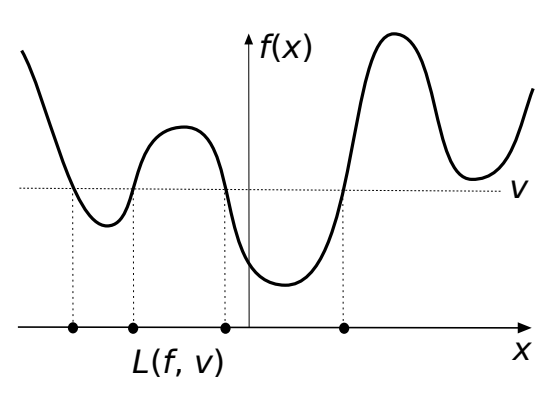
\includegraphics[scale=0.4]{figures/1/3-levelsets.png}
    \caption{Level set}
    \label{fig:levelsets}
\end{figure}
\begin{figure}
    \centering
    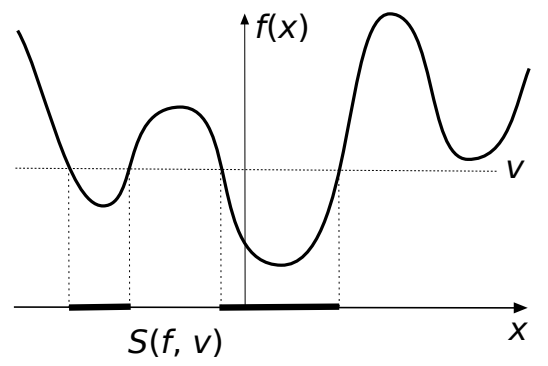
\includegraphics[scale=0.4]{figures/1/4-sublevelsets.png}
    \caption{Sublevel set}
    \label{fig:sublevelsets}
\end{figure}
\par In case that $f$ is unbounded below, we cannot actually talk about sublevel sets. We can reverse the concept and talk about superlevel sets.
%
\par The first property that we'd like that our functions that we minimise have is continuity.
\begin{definition}
    $f:\mathbb{R}^n \rightarrow \mathbb{R}$ is continuous in $x \in \mathbb{R}^n$ if
    \begin{itemize}
        \item $\{x_i\} \rightarrow x \Rightarrow \{f(x_i) \rightarrow f(x)\}$
        \item $\forall \epsilon > 0\ \exists \delta > 0 : |f(y) - f(x)| < \epsilon\ \forall y \in \mathcal{B}(x,\delta)$
    \end{itemize}
\end{definition}
We say that $f$ is continuous on a set $S \subseteq \mathbb{R}^n$ if it is continuous on each $x \in S$.
\begin{theorem}[Intermediate Value Theorem]
    Suppose we have function $f : \mathbb{R} \rightarrow \mathbb{R}$ continuous on a closed interval $[a,b]$. Then:
    \[
        \forall v : \min \{f(a),f(b)\} \leq v \leq \max \{f(a),f(b)\}\ \exists c \in [a,b] : f(c) = v
    \]
\end{theorem}
All the considerations pointed out so far bring us to the Weistrass extreme value theorem. This theorem is one of the most important in optimisation.
\begin{theorem}[Weistrass Extreme Value Theorem]
Suppose we have a set $X \subseteq \mathbb{R}^n$ compact and a function $f$ that is continuous, then the minimising problem has an optimal solution.
\end{theorem}
From this statement, this theorem doesn't seem to be so meaningful. But, if we exploit a little bit some of the considerations explained so far, we can say that this statement is equivalent to say that: if our set is closed and our function continuous, then all the accumulation points of any minimising sequence are optimal solutions and there is at least one of them.
Up until now, we have understand that having a continuous function is a really great thing and for this reason, in a lot of the methods we'll consider, the basic assumptions will be: a compact set and a continuous function.
But, if we are really lucky, we can ask for more. More we have, simpler it is to gain better results.
Talking about continuity, a more strict version of it is Lipschitz continuity.
\begin{theorem}[Lipschitz continuity]
\[
    \exists L > 0 \quad \forall x,y \in X : |f(x) - f(y)| \leq L \lVert x - y \rVert 
\]
\end{theorem}
Since this is a stronger definition of continuity, all the considerations said so far for the continuity case are still true. Moreover, with L continuity, we know that our function doesn't jump wildly. This is a very good result, but unfortunately, a lot of functions are not L continuous. If this is the case, we could see if our function is lower semi continuous (or upper).
%
\par Now, we have to remember our main task: find the minimum of an iterative sequence. For simplicity, we focus our attention on functions in two dimensions. We know that a derivative gives us a linear approximation of the function in that point. So, if I compute the derivative in $x$, in which way of the linear approximation ($f'(x)$) should I go? Of course, we have to go where the line decrease: if the slope of my line is greater than zero, I have to go left, otherwise right. I can stop to iterate when I find $f'(x)=0$ (since I know that in this case we are on a saddle point or a max or min).
\par The saddest part of it is that not all the function have a first derivative and that even if they have it, it may be the case that it isn't continuous. In order to understand when a function is differentiable or not, the definition of derivative is necessary: TODO



\subsection{Useful results about derivatives}
\begin{figure}
    \centering
    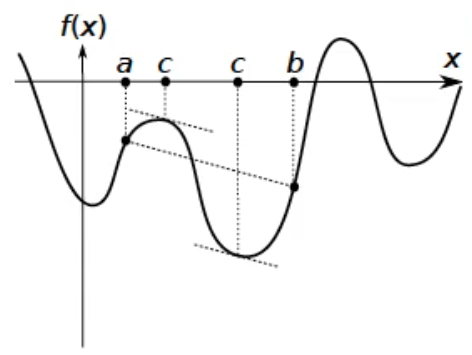
\includegraphics[scale=0.3]{figures/1/chapter1-mean_value_theorem1.png}
    \caption{A differentiable function $f(x)$ and two points $a$ and $b$.}
    \label{fig:chapter1-mean_value_theorem1}
\end{figure}
\par Suppose you have a differentiable function like in figure \ref{fig:chapter1-mean_value_theorem1}, with two points and a line connecting those two points. Then according to the \textbf{mean value theorem} we have the following:
\begin{theorem}
    Given a function $f : \mathbb{R} \rightarrow \mathbb{R}$ continuous on $[a,b]$ and differentiable on $(a,b)$ then there exists a point $c \in (a,b)$ such that the slope of the derivative in point $c$ is the same of the slope of the line connecting $a$ and $b$. In other words:
    \[
        f'(c) = \frac{f(b)-f(a)}{b-a} = m
    \]
    where $m$ is the usual slope of a line.
\end{theorem}
Why do we care about this simple theorem? Because there is a special case of it, namely when $f(a) = f(b)$. This takes the name of \textbf{Rolle's theorem} (see figure \ref{fig:chapter1-rolles_theorem1}) and it says:
\begin{theorem}
    Given a function $f : \mathbb{R} \rightarrow \mathbb{R}$ continuous on $[a,b]$ and differentiable on $(a,b)$, if $f(a) = f(b)$ then there exists a point $c \in (a,b)$ such that the slope of the derivative in point $c$ equals 0.
\end{theorem}
\begin{figure}
    \centering
    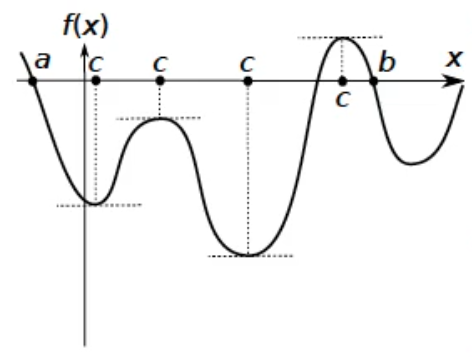
\includegraphics[scale=0.3]{figures/1/chapter1-rolles_theorem1.png}
    \caption{Rolle's theorem.}
    \label{fig:chapter1-rolles_theorem1}
\end{figure}
This theorem assures us that if $f(a) = f(b)$ in the middle there must me at least one local minimum or maximum, or both.
\par Actually, we can even state that between two consecutive roots of $f$ there is an odd number of roots of the derivative $f'$ in the range of $(a,b)$. If $a$ and $b$ are two consecutive roots of $f$ then the sign of their derivatives are opposite to each other.
\par \textit{Exercise}. Prove that between two consecutive roots of $f'$ there is at most one root of $f$.
\par Suppose $a$ and $b$ are two consecutive roots of $f'$. Suppose now by contradiction that there are two different points $c,d \in (a,b)$ that are also the roots of $f$. According to Rolle's theorem, there must exist at least one point $e \in (c,d)$ such that $f'(e)=0$. This contradicts the fact that $a$ and $b$ are two consecutive roots of $f'$.

\subsection{A different interpretation of the gradient}
\par Remember that the function is a mathematical object that lives in $\mathbb{R}^{n+1}$. The gradient is the linear function approximating $f$ in a point. Thus, the gradient it self lives again in $\mathbb{R}^{n+1}$. It is important also to look at it from the input space, i.e. in $\mathbb{R}^n$. We can do that via level sets again.
\par The gradient turns out to be \textit{normal} to the level sets. In other words, it is tangent to the level set.
\subsection{Vector valued function}